\chapter{Теорема об изменении кинетического момента для механической системы.
Законы сохранения кинетических моментов. Дифференциальное уравнение
вращательного движения твердого тела вокруг неподвижной оси. Физический
маятник.}

Теорема об изменении кинетического момента механической системы при ее движении
вокруг неподвижного центра формулируется следующим образом:

полная производная по времени от вектора кинетического момента механической
системы относительно некоторого неподвижного центра \( O \) по величине и
направлению равна главному моменту внешних сил, приложенных к механической
системе, определенному относительно того же центра:
\[
    \der{\vec{K}_O}{t} = \vec{M}^e_O, \text{ где }
    \vec{M}^e_O = \sum_{k=1}^N \vec{m}_O(\vec{F}^e_k) =
    \sum_{k=1}^N \vec{r}_k\times\vec{F}^e_k \text{ --}
\]
главный момент всех внешних сил относительно центра \( O \).

Для системы кинетический момент равен векторной сумме кинетических моментов
всех точек, входящих в систему: \( \vec{K}_O = \sum \vec{M}_{O_j} \). 
Запишем для произвольной точки, входящей в систему, теорему об изменении
кинетического момента:
\[
    \der{}{t} \vec{k}_{O_j} = \vec{m}^e_{O_j} +
    \vec{m}^i_{O_j}.
\]
Суммируя по всем точкам:
\[
    \der{}{t}\sum \vec{k}_{O_j} = \sum \vec{m}^e_{O_j}
    + \underbrace{\sum \vec{m}^i_{O_j}}_0, \text{ откуда }
    \der{\vec{K}_O}{t} = \vec{M}^e_O, \text{ где }
    \vec{M}^e_O = \sum \vec{m}^e_{O_j}.
\]

Производная по времени от кинетического момента системы относительно некоторого
центра равна главному моменту внешних сил относительно этого центра.

В проекциях на оси координат:
\[
    \der{K_x}{t} = M^e_x, \quad\der{K_y}{t} = M^e_y, \quad\der{K_z}{t} = M^e_z.
\]

Частные случаи теоремы:
\begin{enumerate}
    \item Если \( \vec{M}^e_O = 0 \), то \( \vec{K}_O = \const =
    \vec{K}_{O_\text{нач}} \).
    \item Если \( M^e_x = 0 \), то \( K_x = \const = K_{x_\text{нач}} \).
\end{enumerate}
В этих случаях выполняется закон сохранения кинетического момента системы.

\section{Дифференциальное уравнение вращательного движения твердого тела вокруг
неподвижной оси}
Пусть твердое тело вращается вокруг неподвижной оси под действием внешних сил.
В этом случае тело имеет одну степень свободы (\( s = 1 \)) и за обобщенную
координату примем угол поворота (\( q = \phi \)).

Кинетическая энергия тела будет:
\( \ds T = \frac{I_z\omega^2}{2} = \frac{I_z\dot{\phi}^2}{2} \), 
где \( I_z \) -- момент инерции тела относительно оси вращения \( z \).

Обобщенную силу \( Q \) найдем из формулы
\( \delta A = Q\delta q = M_z\delta\phi \), где \( М_z \) -- главный момент
приложенных к телу внешних сил относительно оси \( z \). Имеем \( Q = M_z \).
Подставляя в уравнение Лагранжа второго рода получим дифференциальное уравнение
вращательного движения твердого тела вокруг неподвижной оси:
\( I_z\ddot{\phi} = M_z \).

\section{Физический маятник}
\begin{minipage}{.35\textwidth}
    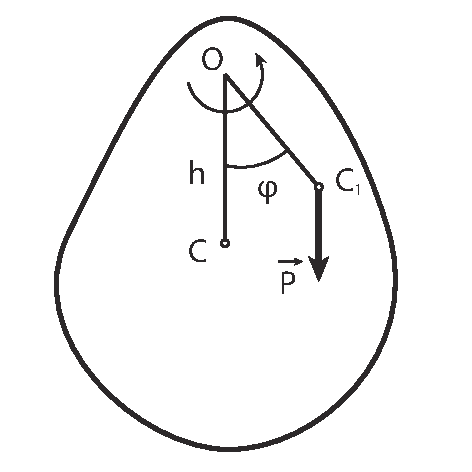
\includegraphics[width=\textwidth]{49_02}
\end{minipage}
\begin{minipage}{.6\textwidth}
Физическим маятником называется твердое тело любой формы, имеющее горизонтальную
ось вращения, не проходящую через центр тяжести тела, называемую осью подвеса.
Рассмотрим движение физического маятника под действием силы тяжести
\( \vec{P} \). Дифференциальное уравнение движения физического маятника будет
\( I_O\ddot{\phi} = -Ph\sin\phi \), где \( I_O \) -- момент инерции маятника
относительно оси вращения \( O \), \( h \) -- расстояние центра инерции \( C \)
от оси вращения (длина физического маятника).
\end{minipage}

При малых колебаниях маятника или при малых углах отклонения \( \phi \) можно
принять \( \sin\phi \approx \phi \), тогда
\[
    I_O\ddot{\phi} = -Ph\phi \text{ или } \ddot{\phi} + \omega^2\phi = 0,
    \text{ где } \omega^2 = Ph/I_O.
\]

Интегрируя это уравнение, найдем \( \phi = C_1\cos\omega t + C_2\sin\omega t \),
где постоянные интегрирования \( C_1 \) и \( C_2 \) определим из начальных
условий движения. Например, пусть при \( t = 0 \) \( \phi_0 = \alpha \),
\( \dot{\phi}_0 = 0 \). Тогда \( \phi =\alpha\cos\omega t \).

Следовательно, под действием силы тяжести (без учета силы сопротивления среды)
маятник совершает гармонические колебания. Частота этих колебаний равна
\( \omega \). Период \( T \) малых колебаний физического маятника равен
\( 2\pi/\omega \).

\newpage
